\documentclass{article} % For LaTeX2e
\usepackage{nips14submit_e,times}
\usepackage{amsmath}
\usepackage{amsthm}
\usepackage{amssymb}
\usepackage{mathtools}
\usepackage{hyperref}
\usepackage{url}
\usepackage{algorithm}
\usepackage[noend]{algpseudocode}
%\documentstyle[nips14submit_09,times,art10]{article} % For LaTeX 2.09

\usepackage{graphicx}
\usepackage{caption}
\usepackage{subcaption}

\def\eQb#1\eQe{\begin{eqnarray*}#1\end{eqnarray*}}
\def\eQnb#1\eQne{\begin{eqnarray}#1\end{eqnarray}}
\providecommand{\e}[1]{\ensuremath{\times 10^{#1}}}
\providecommand{\pb}[0]{\pagebreak}
\DeclarePairedDelimiter\ceil{\lceil}{\rceil}
\DeclarePairedDelimiter\floor{\lfloor}{\rfloor}

\newcommand{\E}{\mathrm{E}}
\newcommand{\Var}{\mathrm{Var}}
\newcommand{\Cov}{\mathrm{Cov}}

\def\Qb#1\Qe{\begin{question}#1\end{question}}
\def\Sb#1\Se{\begin{solution}#1\end{solution}}

\newenvironment{claim}[1]{\par\noindent\underline{Claim:}\space#1}{}
\newtheoremstyle{quest}{\topsep}{\topsep}{}{}{\bfseries}{}{ }{\thmname{#1}\thmnote{ #3}.}
\theoremstyle{quest}
\newtheorem*{definition}{Definition}
\newtheorem*{theorem}{Theorem}
\newtheorem*{lemma}{Lemma}
\newtheorem*{question}{Question}
\newtheorem*{preposition}{Preposition}
\newtheorem*{exercise}{Exercise}
\newtheorem*{challengeproblem}{Challenge Problem}
\newtheorem*{solution}{Solution}
\newtheorem*{remark}{Remark}
\usepackage{verbatimbox}
\usepackage{listings}
\usepackage{mathrsfs}
\title{ProbLimI: \\
Pset I}


\author{
Youngduck Choi \\
CIMS \\
New York University\\
\texttt{yc1104@nyu.edu} \\
}


% The \author macro works with any number of authors. There are two commands
% used to separate the names and addresses of multiple authors: \And and \AND.
%
% Using \And between authors leaves it to \LaTeX{} to determine where to break
% the lines. Using \AND forces a linebreak at that point. So, if \LaTeX{}
% puts 3 of 4 authors names on the first line, and the last on the second
% line, try using \AND instead of \And before the third author name.

\newcommand{\fix}{\marginpar{FIX}}
\newcommand{\new}{\marginpar{NEW}}

\nipsfinalcopy % Uncomment for camera-ready version

\begin{document}


\maketitle

\begin{abstract}
This work contains solutions to the exercises of the problem set I.
\end{abstract}

\bigskip

\begin{question}[1]
\hfill
\begin{figure}[h!]
  \centering
    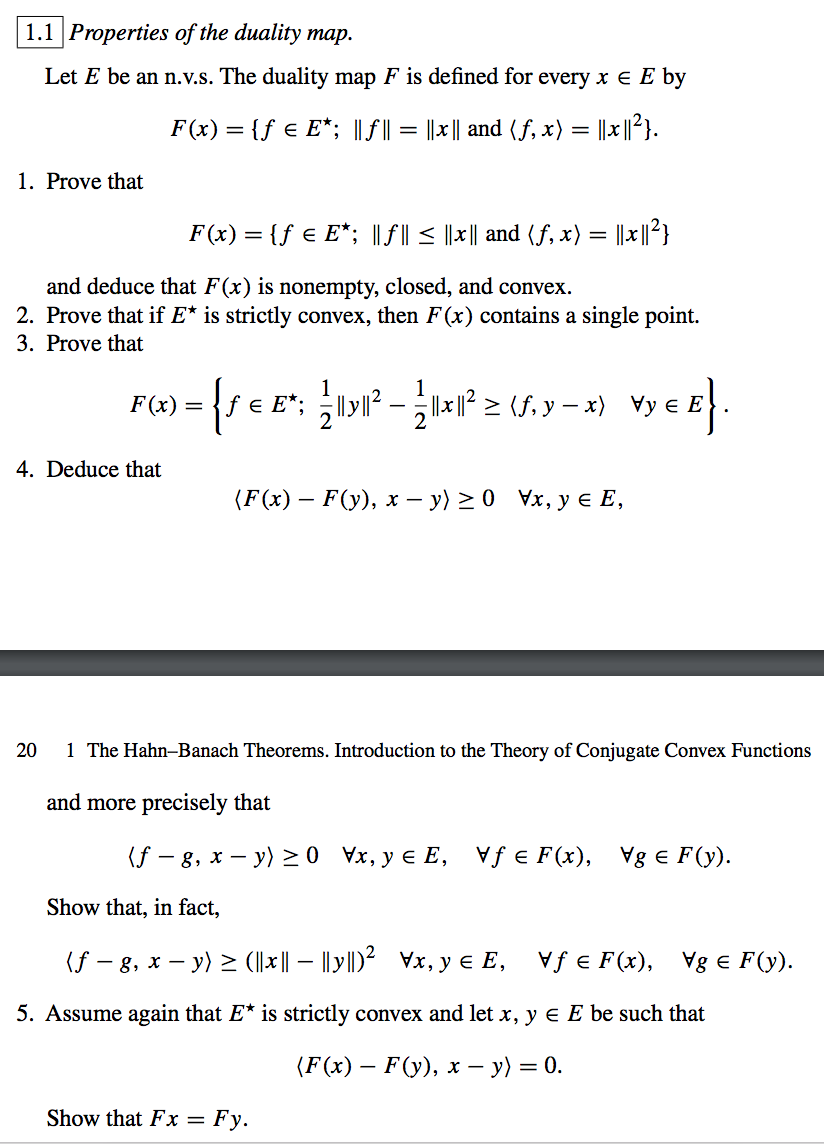
\includegraphics[width=0.7\textwidth]{funcA-1-1.png}
\end{figure}
\end{question}
\begin{solution} \hfill \\
\textbf{(1)} The first set equality follows as 
\eQb
f \in E^* \>\>\> \text{ and} \>\>\> < f, x >  \> = ||x||^2 \implies ||f|| \geq ||x||,
\eQe
because otherwise 
\eQb
|<f , x>| &=& ||x||^2 > ||f|||x||,
\eQe
which is absurd. Now, by Corollary 1.3, it follows that $F(x)$ is non-empty.

\smallskip 
 
We show that $F(x)$ is convex. Let $f,g \in F(x)$ and $t \in [0,1]$. Then,
it follows that
\eQb
< t f + (1-t)g, x> &=& t<f,x> + (1-t)<g,x> = ||x||^2 
\eQe 
and
\eQb
||t f + (1-t)g|| &\leq& t||f|| + (1-t)||g|| \leq ||x||,
\eQe
so $tf + (1-t)g \in F(x)$ and $F(x)$ is convex. 

\smallskip

We show that $F(x)$ is closed. Let $f \in E^*$ such that there exists $\{f_n\} \subset
F(x)$ with $f_n \to f$. As convergence in dual norm implies pointwise convergence,
we have
\eQb
||x||^2 = <f_n, x> \to <f,x> \>\> \text{ and } \>\> <f,x> = ||x||^2. 
\eQe
Also, as $||f_n - f|| \to 0$, and by reverse-triangle inequality, we have
\eQb
||f_n|| \to ||f|| \>\> &\text{and}& \>\> ||f|| \leq ||x||, 
\eQe 
which shows that $f \in F(x)$, and consequently that $F(x)$ is closed.

\bigskip

\textbf{(2)} 

\end{solution}

\newpage


\begin{question}[2]
\hfill
\begin{figure}[h!]
  \centering
    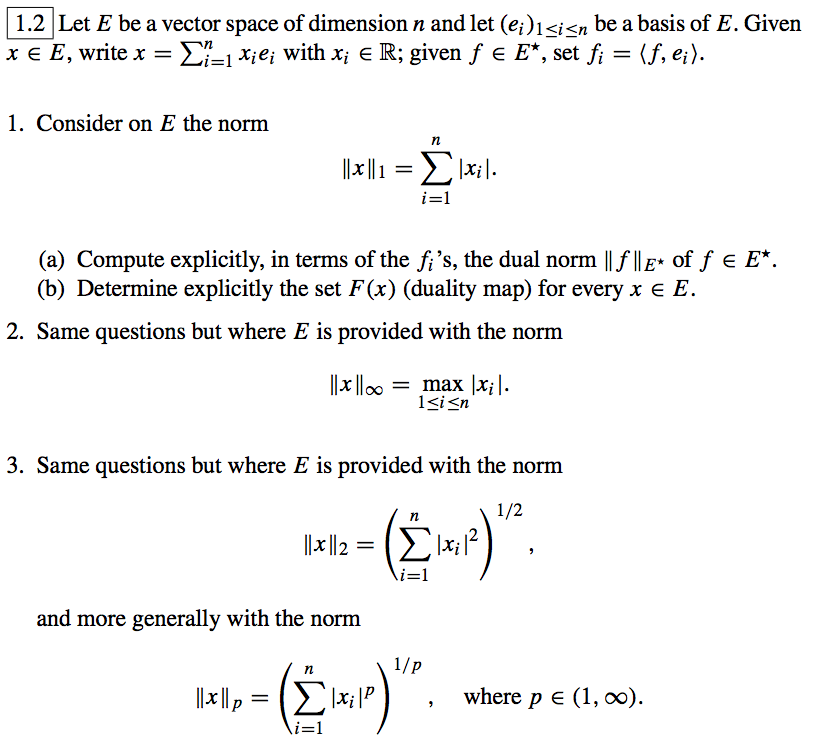
\includegraphics[width=0.7\textwidth]{funcA-1-2.png}
\end{figure}
\end{question}
\begin{solution} \hfill \\
\end{solution}

\newpage

\begin{question}[3]
\hfill
\begin{figure}[h!]
  \centering
    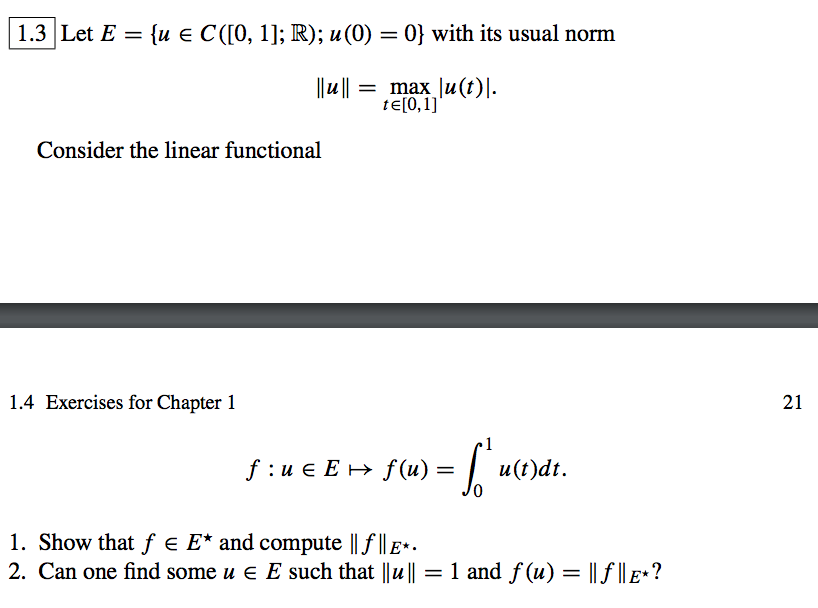
\includegraphics[width=0.7\textwidth]{funcA-1-3.png}
\end{figure}
\end{question}
\begin{solution} \hfill \\
\textbf{(1)}
By linearity of integration, it follows that $f$ defined is linear. Since $f$
is linear, it suffices to show continuity at $0$. Fix $\epsilon > 0$. Then, 
it follows that, with $\delta = \dfrac{\epsilon}{2}$,
\eQb
u \in B(0,\delta) &\implies& |\int_{0}^{1} u(t) dt| \leq 
\int_{0}^{1} |u(t)| dt \leq \delta < \epsilon.
\eQe
Therefore $f$ is continuous. Now, we compute its dual norm explicitly. Note that,
for any $u \in E$,
\eQb
|<f,u>| &=& | \int_{0}^{1} u(t) dt|  \leq \int_{0}^{1} |u(t)| dt  \leq ||u||,
\eQe
so $||f|| \leq 1$. We now show the reverse inequality. Recall that
\eQb
||f|| &=& \sup_{||u|| = 1} |<f,u>|  \\ 
\eQe 
Fix $\epsilon > 0$. Set $u \in C[0,1]$ by
\eQb
t \to \dfrac{1}{\epsilon}X_{[0,\epsilon]}(t) + X_{(\epsilon,1]}(t) \>\> (t \in [0,1]) 
\eQe 
Then, it follows that
\eQb
<f,u> &=& \int_{0}^{1} u(t) dt = 1 - \dfrac{\epsilon}{2}.
\eQe
Therefore, it follows that $||f|| \geq 1$, and we have completed in showing that
$||f|| = 1$. \hfill $\qed$

\bigskip

\textbf{(2)} 

\end{solution}

\newpage

\begin{question}[4]
\hfill
\begin{figure}[h!]
  \centering
    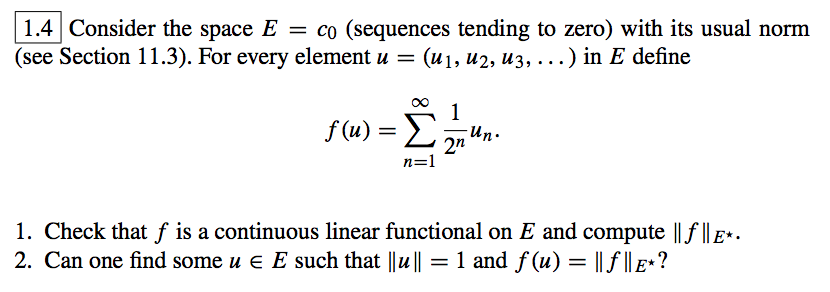
\includegraphics[width=0.7\textwidth]{funcA-1-4.png}
\end{figure}
\end{question}
\begin{solution} \hfill \\
\textbf{(1)} Fix $u \in C_0$ such that 
$||u|| = \sup_n |u_n| = 1$, it follows that 
\eQb
| u_n | &\leq& 1
\eQe 
for all $n \geq 1$, so
\eQb
|f(u)| \leq & \sum_{n=1}^{\infty} |\dfrac{1}{2^n} u_n| = 1. 
\eQe 
Therefore, 
\eQb
||f|| &=& \sup_{||u| = 1} |f(u)| \leq 1. 
\eQe
Now, fix $\epsilon > 0$. Choose $N > 1$ such that 
\eQb
n \geq N \implies \sum_{k=1}^{n} \dfrac{1}{2^k} > 1- \epsilon.
\eQe
Set $u \in c_0$ as 
\eQb
u &=& 1 \>\> (n \leq N) \>\> \text{and} \>\> u =  0 \>\> (n > N).
\eQe
Then, $u \in c_0$, $||u|| = 1$, and $|f(u)| > 1 - \epsilon$. Therefore,
it follows that
\eQb
1 - \epsilon < ||f||
\eQe 
for any $\epsilon > 0$, so $||f|| \geq 1$, which combined with the previous
estimate gives $||f|| = 1$. \hfill $\qed$ 

\bigskip

\textbf{(2)} Suppose for sake of contradiction that there exists $u \in c_0$, such that
\eQb
||u|| = 1 \>\> \text{and} \>\> f(u) = 1.
\eQe
Choose $N > 1$ such that 
\eQb
n \geq N \>\> &\implies& \>\>  u_n < \dfrac{1}{2}.
\eQe
Then,
\eQb
f(u) &<& \sum_{n=1}^{N-1} \dfrac{1}{2^n} u_n  + \dfrac{1}{2} 
\sum_{n=N}^{\infty}\dfrac{1}{2^n} = 
\sum_{n=1}^{N-1} \dfrac{1}{2^n} u_n + \dfrac{1}{2^{N-1}}. \\ 
\eQe
Since $||u|| = 1$, continuing the above estimate gives
\eQb
f(u) &<& 1 - \dfrac{1}{2^{N-1}} + \dfrac{1}{2^{N-1}} = 1, 
\eQe
which is absurd. \hfill $\qed$

\end{solution}

\newpage

\begin{question}[6]
\hfill
\begin{figure}[h!]
  \centering
    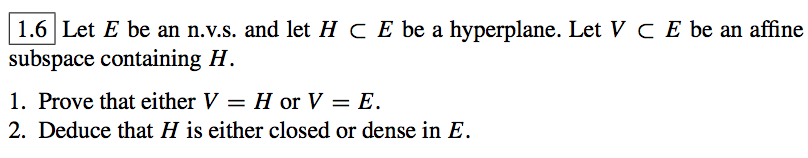
\includegraphics[width=0.7\textwidth]{funcA-1-6.png}
\end{figure}
\end{question}
\begin{solution} \hfill \\
We first show that $\overline{C}$ is convex. Let $x,y \in \overline{C}$, and
$t \in [0,1]$. Choose, $\{x_n\}, \{y_n\} \subset C$ such that $x_n \to x$ and
$y_n \to y$. By convexity of $C$, and linearity of limit, it follows that 
\eQb
\{ tx_n + (1-t)y_n \} \subset C \>\> \text{ and } \>\> 
tx_n + (1-t)y_n \to tx + (1-t)y.
\eQe
Therefore, $tx + (1-t)y \in C$, which proves the convexity of $\overline{C}$.
\end{solution}

\newpage

\begin{question}[7]
\hfill
\begin{figure}[h!]
  \centering
    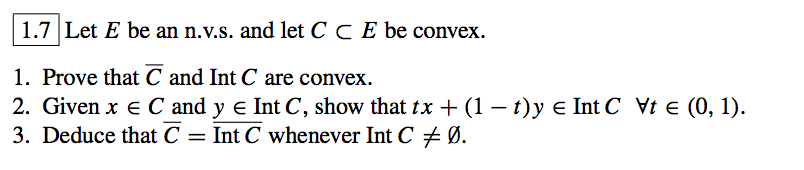
\includegraphics[width=0.7\textwidth]{funcA-1-7.png}
\end{figure}
\end{question}
\begin{solution} \hfill \\
\textbf{(1)}
We first show that $\overline{C}$ is convex. Let $x,y \in \overline{C}$, and
$t \in [0,1]$. Choose, $\{x_n\}, \{y_n\} \subset C$ such that $x_n \to x$ and
$y_n \to y$. By convexity of $C$, and linearity of limit, it follows that 
\eQb
\{ tx_n + (1-t)y_n \} \subset C \>\> \text{ and } \>\> 
tx_n + (1-t)y_n \to tx + (1-t)y.
\eQe
Therefore, $tx + (1-t)y \in \overline{C}$, 
which proves the convexity of $\overline{C}$. We now show that $\int C$ is
convex. Let $x,y \in \int {C}$, and $t \in [0,1]$. By convexity of $C$, 
\eQb
tx + (1-t)y \in C 
\eQe 


\bigskip
We now show that $\int C$ is convex. Let $x,y \in \text{int}{C}$ and $t \in (0,1)$. 



\textbf{(2)} Suppose $x \in C$, $y \in \int C$, and $t \in (0,1)$.  

\bigskip

\textbf{(3)} It is trivial that $\overline{\text{int} C} \subset \overline{C}$. Hence,
it suffices to show that $\overline{C} \subset \overline{\int C}$. 


\end{solution}

\newpage

\begin{question}[8]
\hfill
\begin{figure}[h!]
  \centering
    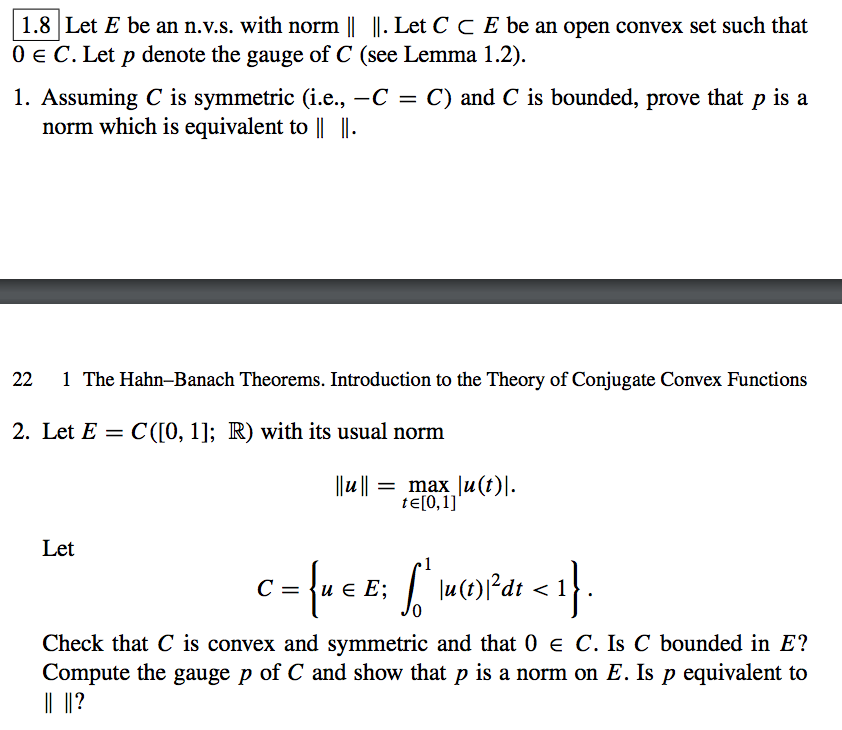
\includegraphics[width=0.7\textwidth]{funcA-1-8.png}
\end{figure}
\end{question}
\begin{solution} \hfill \\
\textbf{(1)}
We first show that $p$ is in fact a norm. By properties of any gauge of $C$,
it suffices to show 
\eQb
p(x) = 0 \>\> &\iff& \>\> x = 0. 
\eQe
If $x = 0$, then 
\eQb
\alpha > 0 \implies a^{-1}x = 0 \in C, 
\eQe
so $p(x) = 0$. Conversely, suppose that $p(x) = 0$. Firstly, let 
\eQb
I &=& \{\lambda > 0 \>;\> \lambda^{-1}x \in C \}, \> \text{ and } \>
0 < \alpha < \beta. 
\eQe
We claim that 
\eQb
\beta \not\in I &\implies \alpha \not\in I.
\eQe
We prove the contrapositive. Suppose $\alpha \in I$. Then, $\alpha^{-1}x \in C$.
By convexity of $C$, it follows that
\eQb
\dfrac{\beta^{-1}}{\alpha^{-1}}\alpha^{-1}x + (1-\dfrac{\beta^{-1}}{\alpha^{-1}})0
&=& \beta^{-1}x \in C,
\eQe
so $\beta \in I$. Therefore, to prove $p(x) > 0$, it suffices to show that
there is a constant $k > 0 $ such that $k^{-1}x \not\in C$.  
Now, suppose for sake of contradiction that $x \neq 0$. 
 Choose $r$ large enough
such that $C \subset B(r,0)$ strictly. Then, 
\eQb
\dfrac{r}{||x||}x \in C \>\> \text{ and} \>\> 0 < \dfrac{||x||}{r} \in I,
\eQe
which as discussed above implies that $p(x) > 0$. Hence, $x = 0$ as required. 

\bigskip

\textbf{(2)} We claim that $C$ is not bounded. Fix $r > 0$. Set 
\eQb
f &=& \sqrt{t} X_{[0,\frac{1}{2r}]} + (r -\sqrt{t})X_{(\frac{1}{2r},\frac{1}{r}]} 
\eQe

\end{solution}

\newpage

\begin{question}[9]
\hfill
\begin{figure}[h!]
  \centering
    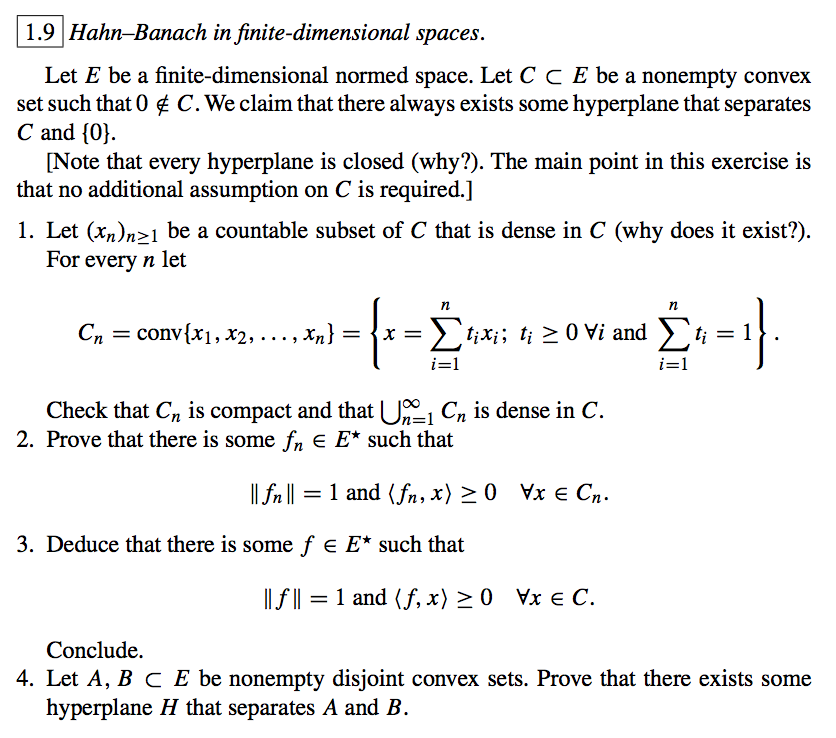
\includegraphics[width=0.7\textwidth]{funcA-1-9.png}
\end{figure}
\end{question}
\begin{solution} \hfill \\
We first note that every hyperplane is closed, because linearity of a map
defined on a finite dimensional space implies continuity. 

\bigskip

\textbf{(1)}

\bigskip

\textbf{(2)}

\bigskip

\textbf{(3)}

\bigskip

\textbf{(4)} Set $C = A - B$. As $ A \cap B = \empty$, we see that $0 \not\in C$. 
We now show that $C$ is still convex. Suppose $x,y \in C$ and $t \in [0,1]$. 
Then, there are $a_x, a_y \in A$ and $b_x, b_y \in B$ such that 
\eQb
x = a_x - b_x \>\> \text{ and } \>\> y = a_y - b_y. \\
\eQe
Then, it follows that
\eQb
tx + (1-t)y &=& t(a_x - b_x) + (1-t)(a_y - b_y) = (ta_x + (1-t)a_y) - 
(tb_x - (1-t)b_y) \in C,
\eQe
where the last inclusion holds by convexity of $A$ and $B$. Hence, $C$ is a 
nonempty convex set such that $0 \not\in C$. Apply $(3)$ to $C$, then
there is $f \in E^*$ such that 
\eQb
<f,x> 
\eQe

\end{solution}

\newpage

\begin{question}[10]
\hfill
\begin{figure}[h!]
  \centering
    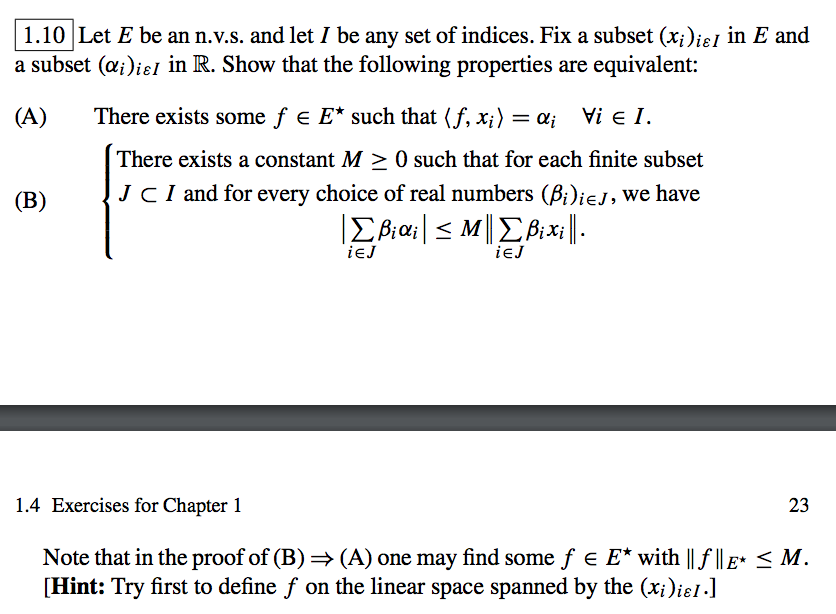
\includegraphics[width=0.7\textwidth]{funcA-1-10.png}
\end{figure}
\end{question}
\begin{solution} \hfill \\
ddd
\end{solution}
\newpage

\begin{question}[11]
\hfill
\begin{figure}[h!]
  \centering
    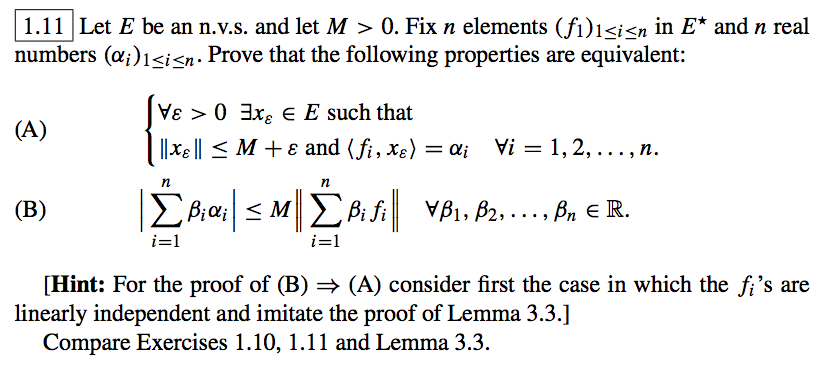
\includegraphics[width=0.7\textwidth]{funcA-1-11.png}
\end{figure}
\end{question}
\begin{solution} \hfill \\
ddd
\end{solution}

\end{document}

